\scanpage{93}\mspage{84}
L'axiome de divisibilité \deleted{\unsure{équi}} Mag L 1. équivaut ici au fait que \deleted{\unsure{la}} l'ens ordonné soit divisible
\[
\begin{aligned}
 \text{Mag L }1&\Longleftrightarrow \forall S_{a,b},\quad |S_{ab}|^\circ\overset{\text{déf}}{=} ]a,b[\ne\varnothing\\
 &\qquad\text{i.e. si }a<b,\ \exists x\ \text{avec}\ a<x<b.
\end{aligned}
\]

Cela implique-t-il Mag L 2 ? \deleted{Non, exemple}

\[
\begin{aligned}
 \substack{\text{Mag L 2 signifie}\\\text{ici deux choses}}\quad
 \left|\begin{aligned}
 a)&\ \text{pour }P_x,S_{a,b}:\quad
     x\parallel\deleted{\unsure{\{} }]a,b[\ \Longrightarrow x\leq a\ \text{ou}\ x\geq b\\
 &\quad\deleted{\Longrightarrow\text{ ou encore }x\parallel\{a,b\}}\\
 b)&\ \text{pour }S_{a,b},S_{a',b'}\quad
      ]a,b[\deleted{\unsure{\bullet}}\mathrel{\unsure{\mid\cdot\mid|\parallel}}]a',b'[
         \Longrightarrow b\leq a'\ \text{ou}\ b'\leq a
 \end{aligned}\right.
\end{aligned}
\]
mais b) résulte en réalité de a) \deleted{\unsure{ou encore}} \deleted{$\Rightarrow\ \unsure{\{a,b\}}\parallel ]a',b'[$, et \unsure{on applique} a)}

\deleted{Dans les deux cas, il faut \unsure{préciser|prouver}}

\uline{Lemme} \deleted{\unsure{Il}}Pour que Mag L 2 soit valable, il f et s. que \inserted{(i) $L$ soit div.} \inserted{et} que \inserted{\deleted{\unsure{(ii)}}} $\forall x\in L$, et $a<b$, on ait
\[
 x\parallel ]a,b[ \Longrightarrow \deleted{x\parallel\{a,b\}} x\leq a\ \text{ou}\ x\geq b.
\]

\deleted{(où pour deux \unsure{parties} une partie $A$ de $L$, on pose}
\[
 \deleted{x\parallel A\Longleftrightarrow\forall y\in A,\quad x\parallel y\quad
         (\text{i.e. } x<y\ \text{ou}\ y<x)}
\]
\deleted{ou encore, que \unsure{s}}
\deleted{a) Si $a\unsure{\notin|\in}L$ n'est pas un plus grand élément, on ait}
\[
 \deleted{L_{\leq a}=\bigcap_{b\in L_{>a}}}
\]

Ou encore, que

\unsure{(iia)|(iii)} a) $\forall a\in L$, t. q. $a$ ne soit pas un plus grand élément, on ait
\[
 \bigcap_{\underset{\sim}{c}>a}L_{\leq c}=L_{\leq a}
\]

b) $\forall b\in L$ tel que $b$ ne soit pas un plus petit élément, on ait
\[
 \bigcap_{\underset{\sim}{c}<b}L_{\geq c}=L_{\geq b}
\]

\unsure{Ce|Ceci} n'est le plus souvent pas satisfait pour les \deleted{\unsure{magmas}} ens. ordonnés associés \deleted{\unsure{aux}}\inserted{à une} corde topologique, exemple
\figure{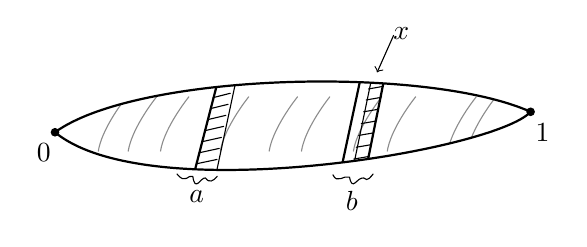
\begin{tikzpicture}[x=1cm,y=1cm,line cap=round,line join=round]
 \begin{scope}
  \clip (0,0) .. controls (1.05,.76) and (4.72,.85) .. (6.04,.26)
       .. controls (5.6,-.23) and (1.19,-.98) .. (0,0);
  \foreach \x in {.70,1.08,1.49,2.25,2.87,3.28,3.94,4.37,5.14,5.39}
     \draw[thin,black!45] (\x-.15,-.24) .. controls (\x-.11,.02) and (\x+.13,.35) .. (\x+.21,.45);
  \draw[thick] (1.71,-.74)--(2.12,.85);
  \draw (2,-.74)--(2.34,.85);
  \foreach \y in {-.53,-.40,-.26,-.12,.02,.16,.30,.44,.58}
     \draw ({1.75+(.59+\y)*.25},\y)--({2.02+(.59+\y)*.20},\y+.055);
  \draw[thick] (3.58,-.72)--(3.91,.82);
  \draw (3.73,-.72)--(4.05,.82);
  \draw[thick] (3.90,-.72)--(4.21,.82);
  \foreach \y in {-.50,-.34,-.19,-.04,.11,.26,.41,.55}
    \draw ({3.74+(.60+\y)*.21},\y)--({3.92+(.60+\y)*.20},\y+.03);
 \end{scope}
 \draw[thick] (0,0) .. controls (1.05,.76) and (4.72,.85) .. (6.04,.26)
       .. controls (5.6,-.23) and (1.19,-.98) .. (0,0);
 \fill (0,0) circle (.055) (6.04,.26) circle (.055);
 \node[below left] at (.07,-.02) {$0$};
 \node[below right] at (5.98,.23) {$1$};
 \draw (1.55,-.53) .. controls (1.66,-.67) and (1.69,-.53) .. (1.75,-.56)
            .. controls (1.78,-.77) and (1.85,-.57) .. (1.91,-.58)
            .. controls (1.96,-.65) and (2.01,-.62) .. (2.06,-.56);
 \node[below] at (1.80,-.62) {$a$};
 \draw (3.53,-.54) .. controls (3.58,-.66) and (3.67,-.54) .. (3.74,-.57)
            .. controls (3.78,-.76) and (3.83,-.57) .. (3.92,-.58)
            .. controls (3.97,-.64) and (4.02,-.55) .. (4.04,-.53);
 \node[below] at (3.77,-.62) {$b$};
 \draw[->] (4.30,1.23)--(4.09,.76);
 \node[above right,inner sep=0pt] at (4.29,1.17) {$x$};
\end{tikzpicture}}
% archive sheet number: 93

